\chapter{Analysis}
In order to accomplish said objectives listed on the problem Statement Analysis, it is first
needed to enlist the embedded system components, this will help to choose a STM32 model as 
well the modules for this task without any over and under dimensions.

\begin{itemize}
    \item Microcontroller \\\hspace*{1cm} The STM32 CPU that will control the Embedded System.
    \item GNSS \\\hspace*{1cm} A module to acquire the world position in latitude and longitude.
    \item Mobile Communication \\\hspace*{1cm} The module with the ability to communicate wirelessly with MongoDB 
    \item Power Source \\\hspace*{1cm} The set of batteries the system will relay on for energy. It is stipulated that
    the system must have the autonomy of at least 30 days.
    \item SD Card Slot \\ Local long term memory in case of field transmission.
    \item Sensors:
    \begin{itemize}
        \item IMU \\\hspace*{1cm} System physical acceleration and angle data.
        \item Temperature Sensor \\\hspace*{1cm} Water Temperature data.
        \item Power Source Level Sensor \\\hspace*{1cm} Voltage reading data.
    \end{itemize}
\end{itemize}

\section{Requirements and Constraints}
\subsection{Requirements}
\begin{itemize}
    \item Search and selection of hardware components.
    \item Software design.
    \item PCB design.
    \item 5S outer shell 3D design.
    \item Actual product realization.
    \item Laboratory tests.
\end{itemize}
\subsection{Constraints}
\begin{itemize}
    \item Limited Team
    \item The project must be presented for evaluation within deadline.
    \item The project has to be validated at the ocean.
    \item The pretended autonomy has to be of a mouth at minimum.
\end{itemize}


\begin{figure}[H]
    \centering
    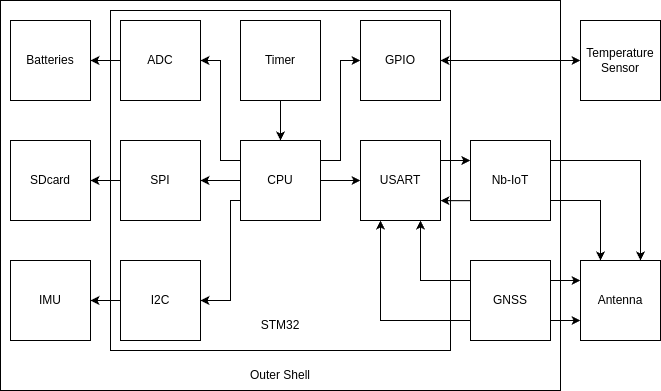
\includegraphics[width=0.9\textwidth]{images/diagrams/block_diagram/block_diagram_2/block_diagram.png}  % Adjust the width as necessary
    \caption{Block Diagram}
    \label{fig:Block Diagram}        
\end{figure}


As for the outer shell there are a few things to have in attention. 

\begin{itemize}
    \item The Antenna to floater distance, once the water interferes with the antenna signal.
    \item The float size, that needs to support all the weight and float, respecting the fisrt topic.
    \item The drifter ballast, that will be the drifter core, located between the 
    floater and the temperature sensor tip. It should be heavy so the drifter points up, but it should't exeed the 
    second topic demand 

\end{itemize}

%corrigir, falta a case no meio e ta mau recortado
\begin{figure}[H]
    \centering
    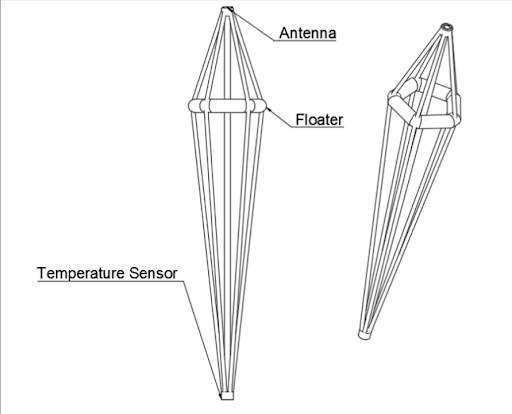
\includegraphics[width=0.7\textwidth]{images/diagrams/shell/unnamed.png}  % Adjust the width as necessary
    \caption{Floater Architecture}
    \label{fig:Floater Architecture}        
\end{figure}

%vila do conde + ou - 10km mar adentro 2g 4g\\
%mapa de alcance na costa\\
%atenção ao clima \\
\section{State of the art}
%%usar fotos do projeto no lab
twretwertw
\subsection{Economy}
twertwert
\subsection{Ecology}
wertwert
\subsection{Sports}
\section{Market Research}



\section{System Architecture}


\subsubsection{Block Diagram}

\begin{figure}[H]
    \centering
    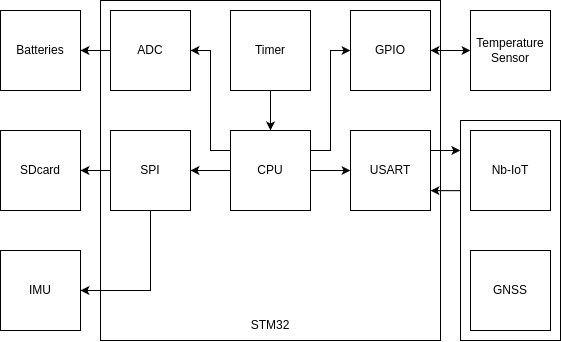
\includegraphics[width=0.7\textwidth]{images/diagrams/block_diagram/block_diagram_1/block_diagram.drawio.png}  % Adjust the width as necessary
    \caption{Block Diagram}
    \label{fig:Block Diagram}        
\end{figure}

\subsubsection{Use Case}

\begin{figure}[H]
    \centering
    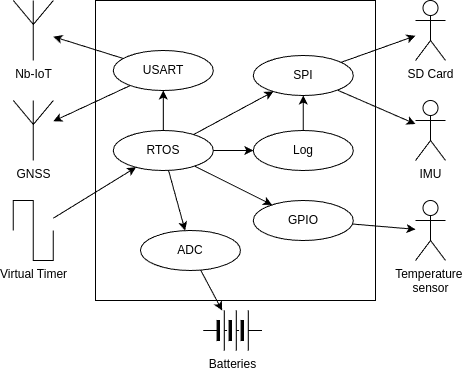
\includegraphics[width=0.7\textwidth]{images/diagrams/use_case/Use Case.drawio.png}  % Adjust the width as necessary
    \caption{Use Case Diagram}
    \label{fig:Use Case Diagram}        
\end{figure}

\subsubsection{Sequence Diagram}

\begin{figure}[H]
    \centering
    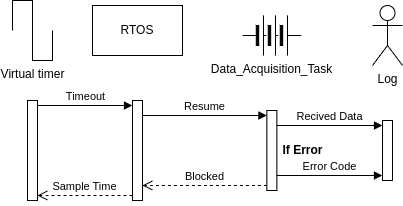
\includegraphics[width=0.7\textwidth]{images/diagrams/sequence_diagram/sequence_diagram_1/Sequence Diagram.drawio.png}  % Adjust the width as necessary
    \caption{Sequence Diagram of Sensor Task}
    \label{fig:Sequence Diagram of Sensor Task}
\end{figure}

\begin{figure}[H]
    \centering
    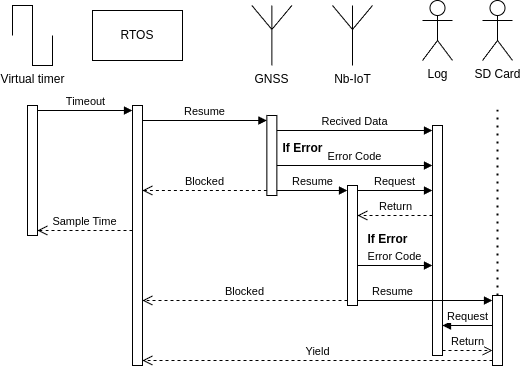
\includegraphics[width=0.7\textwidth]{images/diagrams/sequence_diagram/sequence_diagram_2/Sequence Diagram.drawio.png}  % Adjust the width as necessary
    \caption{Sequence Diagram for Sending and Archive Task}
    \label{fig:Sequence Diagram for Sending and Archive Task}        
\end{figure}

\subsubsection{Threads} 
Once this problem requires a list of taks to be executed, using a OS will allow
a better project organization and performance with little to no impact in power consumption.

As the ST uC offers a variety of RTOS, the implementation will be acessible with good support due to the
CMSIS v2 abstraction layer.

The division in Threads demands a separation in Priority levels, as the OS scheduler takes in consideration 
once both tasks are ready for execution.  

Seting a task priority it must take in vision the resources the task will use, the time it will take to execute said behavior
and the actual importance in matching it time constraints. In order to menage this level of complexity, the RTOS offers a set of
tools for tasks control that will be used for its synchronization and comunication.
\begin{itemize}
    \item High Priority Threads \\ 
    Tasks that will handle the outer communication as GNSS and the internet integration will take the higher priority once, as will be handled
    by a peripheral, its execution will be faster, only using the USART interface for AC transmission. 
    \item Normal Priority Threads \\
    The only task here will be the one that has enough importance to be prioritized over the sensors but as the transmission beggins it should release the processor
    for the outer communication.
    \item Low Priority Threads \\
    Tasks that only has to measure the sensors having no problem to be removed from the CPU execution
    once their execution is, in their majority, asynchronous.
    
\end{itemize}

%rescrever
\begin{figure}[H]
    \centering
    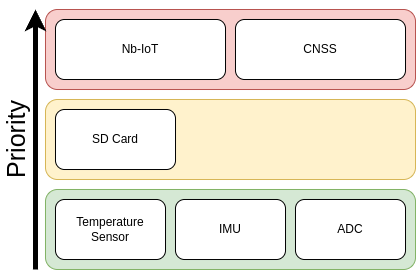
\includegraphics[width=0.7\textwidth]{images/diagrams/threads/thread.drawio.png}  % Adjust the width as necessary
    \caption{Thread Priority Stack}
    \label{fig:Thread Priority Stack}        
\end{figure}


\begin{figure}[H]
    \centering
    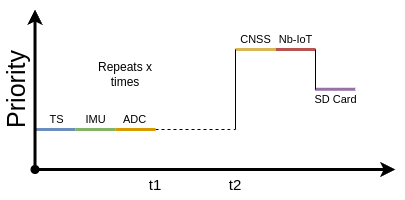
\includegraphics[width=0.7\textwidth]{images/diagrams/threads/graph/threads_graph.drawio.png}  % Adjust the width as necessary
    \caption{Thread Temporal Graph}
    \label{fig:Thread Temporal Graph}        
\end{figure}

\begin{figure}[H]
    \centering
    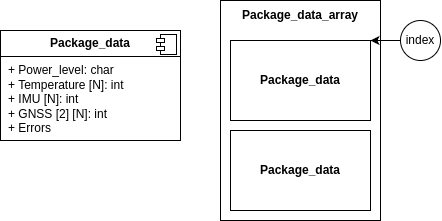
\includegraphics[width=0.7\textwidth]{images/diagrams/data_struct/package_data.drawio.png}  % Adjust the width as necessary
    \caption{Package data structure}
    \label{fig:Package data structure}        
\end{figure}


\begin{figure}[H]
    \centering
    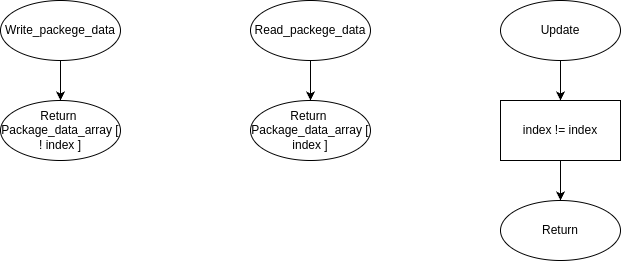
\includegraphics[width=0.7\textwidth]{images/diagrams/data_struct/fluxogram.png}  % Adjust the width as necessary
    \caption{Memory Flowchart}
    \label{fig:Memory Flowchart}        
\end{figure}
